\documentclass[spanish,12pt,a4paper,final,oneside]{book}
\setlength{\parindent}{0pt}
\setlength{\parskip}{0.5em}
\usepackage[spanish]{babel}
\usepackage[utf8]{inputenc}
\usepackage[bottom]{footmisc}
\usepackage[a4paper, total={16cm, 24cm}]{geometry}

\usepackage{longtable}
\setlength{\tabcolsep}{12pt}

\usepackage{amsmath}
\usepackage{amsfonts}
\usepackage{amssymb}

\usepackage{graphicx}
\graphicspath{ {./imagenes/} }

\usepackage[colorlinks]{hyperref}
\hypersetup{colorlinks=true}
\hypersetup{urlcolor=blue}
\usepackage{cleveref}

\usepackage{fancyhdr}
\fancyhf{}
\fancyhead[RE]{\small\scshape\nouppercase{\leftmark}}
\fancyhead[LO]{\small\scshape\nouppercase{\leftmark}}
\fancyhead[LE,RO]{\small\thepage}
\pagestyle{fancy}

\usepackage{authoraftertitle}
\title{}
\author{Juan Murua Olalde}
\date{}

\begin{document}

\section{Mapa resumen de los flujos de información dentro de una empresa digitalizada}
Uno de los principales cambios de mentalidad a que nos obliga la nueva situación es a pensar de forma global. Con la tecnologia actual, la información puede fluir libremente por toda la empresa e incluso por su entorno (proveedores, clientes,...). Es importante no perder de vista el mapa general. Como se suele decir: que los árboles no nos impidan ver el bosque.

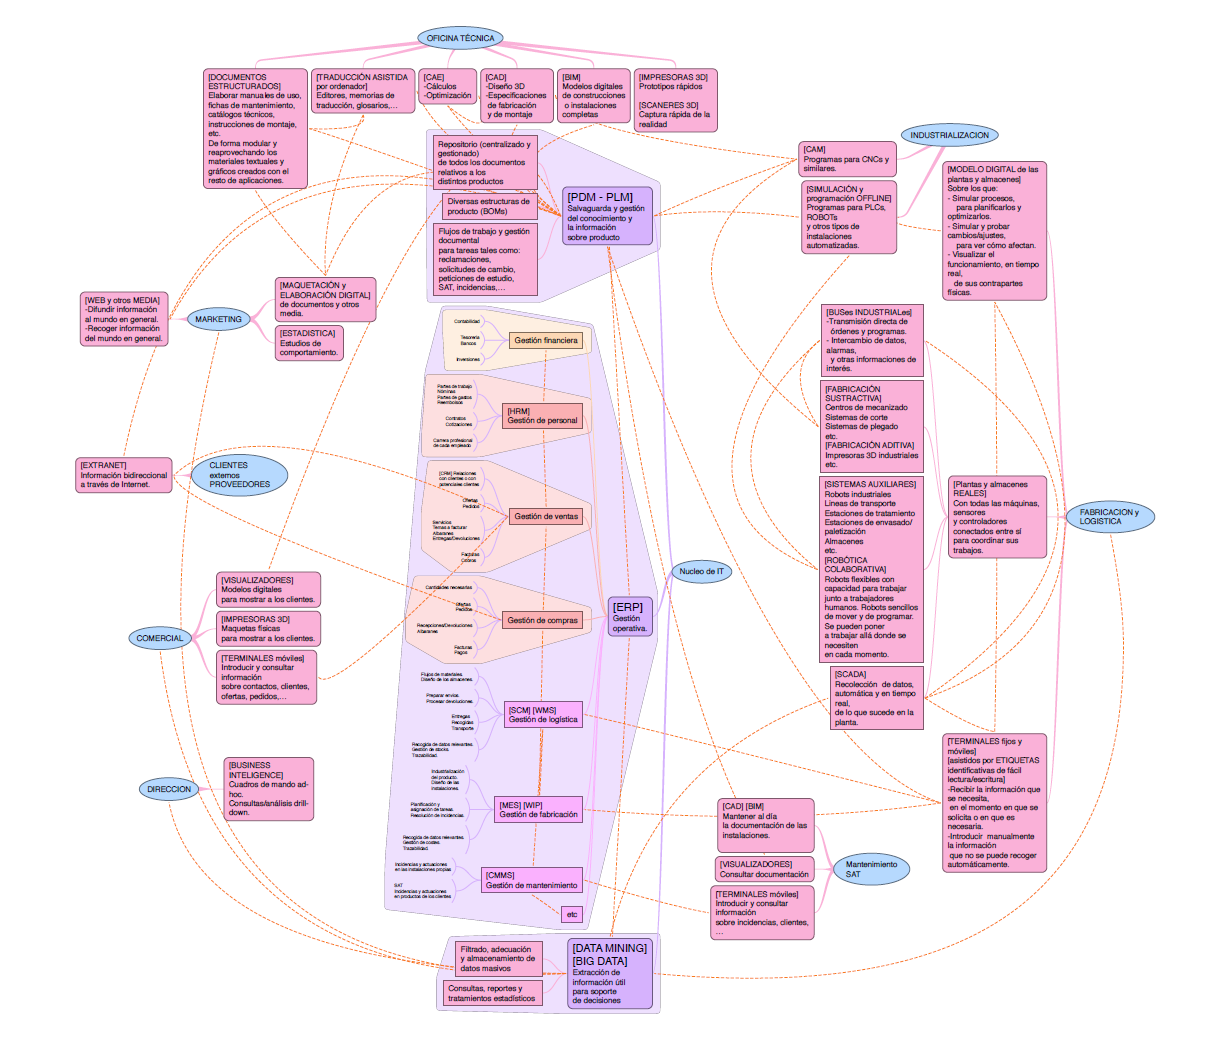
\includegraphics[width=1.1\textwidth]{Empresa_4.0_-_Esquema_general_de_los_flujos_de_informacion_en_una_empresa_digitalizada.png}

El ``bosque'', visto así, puede parecer intimidante. Pero, a medida que vayamos analizando cada una de sus partes y comprendiendo cómo encajan en la globalidad. Se ve que es un maravilloso ecosistema lleno de vida, con múltiples sinergias entre cada una de sus partes y cada uno de sus habitantes. Un ecosistema en constante evolución, donde cada habitante aprende y se va adaptando a las diversas circunstancias que se van presentando.

\subsection{Unos comentarios importantes, que se aplican a todos los apartados siguientes}
Por un lado,  indicar que la principal intención tras el mapa es suministrar un punto de partida para reflexionar. La intención de los apartados en este capítulo es la de desmenuzar el mapa general. Irnos concentrando en puntos concretos del mismo. Mientras vamos pensando en cómo se podria aplicar todo lo citado (y más) en el caso concreto de nuestra empresa.

Conviene pensar en nuestro trabajo habitual, en casos concretos. Para tratar de imaginarnos cómo se podrian desarrollar estos si tuvieramos en todo momento, al alcance de la mano, todos los datos necesarios. (Nota: La reflexión comienza por imaginarnos cuáles son o podrian ser esos ``datos necesarios''. Sin limitarnos solo a los que manejamos en la actualidad.)

Los ejemplos de operaciones que se indican aquí son meramente orientativos. Quien trabaja en cada uno de los departamentos citados pensará en muchas otras operaciones y tareas habituales en su día a día. Lo dicho, esto es un mapa general ilustrativo, no pretende ser algo exhaustivo.

Un par de puntualizaciones prácticas:
\begin{itemize}

\item Cuando se dice ``Registran...'' se quiere decir que cada dato a registrar se guarda en el sistema en el mismo momento en que se tiene conocimiento de él. 
\begin{itemize}
\item Si al registrar algo hay alguna duda, se aplica lo de ‘más vale tener datos incompletos que no tener ningún dato’. Eso sí, se ha de resolver la duda en el menor tiempo posible y completar los datos en cuanto se haya resuelto.
\item Si más tarde se descubre algún error en los datos. La misma persona que lo descubre se encarga de corregirlo. Si alguien habia utilizado el dato erróneo para algo, tendrá que ajustar también su actuación en cuanto detecte la discrepancia. 
\item Es conveniente cruzar información siempre que sea posible (por ejemplo, tener el pedido de compra a la vista siempre que se registra un albarán de recepción). Es conveniente realizar consultas de comprobación cuando se vea algo ‘raro’ o que parezca ‘no cuadrar’ con lo que se espera. 
\end{itemize}

\item Cuando se dice ``Reciben...'' o ``Consultan...'' esa consulta es, obviamente, digital. 
\begin{itemize}
\item El equipamiento informático es barato. Se presupone que hay dispositivos (pantallas) suficientes para que cualquiera que necesite procesar un dato tenga siempre a mano algún dispositivo adecuado para hacerlo.
\item La capacidad de procesamiento de esos dispositivos permite realizar con agilidad búsquedas y análisis sobre la información contenida en el sistema. Se presupone que cada persona tiene la suficiente habilidad en el manejo del sistema como para saber buscar por sí misma lo que necesita en cada momento. (nota: No solamente saber lo habitual, sino también tener suficiente conocimiento general como para resolver situaciones puntuales, o incluso extraordinarias, por sí misma.)
\end{itemize}

\end{itemize}


\subsection{Las personas encargadas de las ventas}

Registran en el ERP la interacción con los clientes (datos, ofertas, pedidos, consultas, incidencias,...). 

Registran en el ERP las listas de precios. Para ello, consultan en el ERP información sobre costes, volumen de pedidos,...

Consultan en el ERP información sobre la disponibilidad de inventarios, las previsiones de fabricación, la carga de trabajo de las personas encargadas de proveer servicios,... Para elaborar y lanzar los despachos de pedidos. 

Reciben notificación de incidencias con los pedidos a servir, incidencias en cobros,... Para gestionarlas y solventarlas.

Cada cliente puede consultar (en el ERP) el estado de sus datos, ofertas, pedidos, consultas, incidencias,... (la parte que se desee compartir con él).

Cada cliente, puede consultar (en el PDM) la información (guias de uso, guias de mantenimiento,...) que necesita para utilizar los productos que ha comprado.

\subsection{Las personas encargadas de las compras}

Registran en el ERP la interacción con los proveedores (datos, ofertas, pedidos, consultas, incidencias,...). 

Consultan en el ERP información sobre la disponibilidad de inventarios, las previsiones de pedidos, las previsiones de fabricación,... Para elaborar y lanzar los pedidos que sean necesarios.

Reciben solicitudes para trasladar a los proveedores consultas sobre posibilidades, precios, disponibilidades,... Responden a los solicitantes con la información recabada.

Cada proveedor puede consultar (en el ERP) el estado de sus datos, ofertas, pedidos, consultas, incidencias,... (la parte que se desee compartir con él).

Cada proveedor subcontratado para fabricar producto, puede consultar (en el PDM) la información (diseño, especificaciones,...) que necesita para fabricarlo.

\subsection{Las personas encargadas del almacenaje\\y de las recepciones/envios de materiales}

Reciben peticiones para servir pedidos o para mover materiales de un almacén a otro.

Registran en el ERP los envios de materiales y los acuses de recibo en destino (si procede). 

Registran en el ERP las recepciones de materiales y las ubicaciones donde quedan almacenados.

Consultan en el ERP los materiales pendientes de recibir o pendientes de enviar en cada almacén.  

Reciben notificación de incidencias con los movimientos de material, con las entregas,... Para gestionarlas y solventarlas.

\subsection{Las personas encargadas de los servicios post-venta}

Reciben peticiones para atender a los clientes. Registran en el ERP los servicios realizados y las incidencias relacionadas con ellos.

En el caso de instalaciones grandes o personalizadas, elaboran y recopilan información detallada para documentar cada instalación. Registran dicha información en el PDM.

Consultan en el PDM información acerca de diseños, especificaciones, manuales de servicio,... de cada producto que han de atender.

\subsection{Las personas encargadas de la fabricación de producto}

Consultan en el ERP información sobre la disponibilidad de inventarios, las previsiones de pedidos, el estado de las compras, la disponibilidad de los recursos productivos,... Para elaborar y lanzar las órdenes de fabricación que sean necesarias.

Registran en el ERP información sobre la ejecución de las órdenes de fabricación.

Reciben notificación de incidencias en los trabajos en curso, en las instalaciones,... Para gestionarlas y solventarlas.

Consultan en el PDM información acerca de diseños, especificaciones, requisitos,... de cada producto que han de fabricar. Con los productos habituales, para guiar el proceso de fabricación. Con los productos nuevos, para elaborar y establecer los procesos de fabricación pertinentes.

Realizan simulaciones acerca de los flujos de materiales en la planta, teniendo en cuenta las capacidades reales de la misma. En el corto plazo, para estudiar el impacto de las incidencias y buscar la mejor forma de solventarlas. En el largo plazo, para mejorar y optimizar los procesos de fabricación.

\subsection{Las personas encargadas de las infraestructuras}

Reciben notificación de incidencias en las instalaciones,... Para gestionarlas y solventarlas.

Consultan en el PDM información acerca de diseños, especificaciones, manuales de servicio,... de cada instalación que han de atender.

Diseñan e implementan mejoras en las instalaciones existentes y ampliaciones con nuevas instalaciones. El diseño y la programación de los nuevos sistemas se realizan sobre un gemelo digital de la planta, reduciendo así el impacto de los cambios cuando estos se han de ejecutar en la planta física real.  Elaboran y recopilan información detallada para documentar cada instalación. Registran y mantienen actualizada toda esa información en el PDM.

\subsection{Las personas encargadas del diseño de producto}

Diseñan nuevos productos y estudian mejoras en los productos existentes. El diseño, los cálculos, los ensayos y las simulaciones se realizan primero sobre modelos digitales y luego sobre prototipos físicos.  Elaboran información detallada para documentar cada producto, incluyendo tanto los aspectos necesarios para su fabricación, como para su servicio, como para su utilización. 

Registran y mantienen actualizada toda esa información en el PDM.

Reciben notificación de peticiones de cambios, incidencias,... Para gestionarlas y solventarlas.

\subsection{Las personas encargadas de la promoción de los productos y servicios que ofrece la empresa}

Consultan en el PDM información acerca de diseños, especificaciones, manuales de servicio, manuales de uso,... de los productos.

Elaboran documentación y materiales multimedia de promoción. 

Elaboran y supervisan la imagen corporativa en todos los documentos que se utilicen fuera de la empresa. Registran y mantienen actualizada toda esa información en el PDM.

Reciben notificación de las incidencias y quejas de los clientes,... Para gestionarlas y solventarlas.

Consultan en el repositorio de datos (DATA MINING, BIG DATA), para elaborar y destilar la información que necesitan para diseñar campañas de publicidad y para tomar decisiones acerca del desarrollo de producto.

(nota: IT se encarga de la captura, filtrado, adecuación y almacenamiento de los datos en bruto. Para que estén disponibles en un formato adecuado para la consulta y elaboración de información por parte de los usuarios, que utilizarán para ello las herramientas de mineria de datos correspondientes.)

\subsection{Las personas encargadas de los cobros y los pagos}

Registran en el ERP las previsiones de necesidades financieras y los movimientos reales de dinero (cobros, pagos, inversiones,...). 

Reciben notificación de incidencias con los pagos, con los cobros,... Para gestionarlas y solventarlas.

Registran en el ERP los preceptivos registros contables y elaboran las cuentas legales.

\subsection{Las personas encargadas de las personas}

Consultan en el ERP los partes de trabajo, partes de gastos,... Para elaborar y liquidar las nóminas y otros pagos.

Reciben notificación de incidencias con las nóminas, las cotizaciones,... Para gestionarlas y solventarlas.

Registran en el ERP los datos relativos a cada empleado.

\subsection{Las personas encargadas de dirigir la empresa}

Consultan en el ERP la información relativa a la marcha de la empresa.

Reciben notificación de incidencias graves,... Para gestionarlas y solventarlas.

Consultan en el repositorio de datos (DATA MINING, BIG DATA), para elaborar y destilar la información que necesitan para tomar decisiones.

(nota: IT se encarga de la captura, filtrado, adecuación y almacenamiento de los datos en bruto. Para que estén disponibles en un formato adecuado para la consulta y elaboración de información por parte de los usuarios, que utilizarán para ello las herramientas de mineria de datos correspondientes.)


\end{document}
